\usepackage{amsthm}

\newtheorem{theorem}{Theorem}[chapter]
\newtheorem{lemma}           [theorem] {Lemma}   
\newtheorem{folg}           [theorem] {Folgerung}   

\newtheorem{frage}       [theorem] {Frage}   
\newtheorem{question}       [theorem] {Question}   
\newtheorem{aufgabe}       [theorem] {Aufgabe}   
\newtheorem{exercise}       [theorem] {Exercise}  

\newtheorem{proposition}     [theorem] {Proposition}  
\newtheorem{satz}     [theorem] {Satz}  
\newtheorem{fact}{Fact}
\newtheorem{definition}      [theorem] {Definition} 

\theoremstyle{definition} 
\newtheorem{bemerkung}     [theorem] {Bemerkung}  
\newtheorem{beispiel}       [theorem] {Beispiel}  
\newtheorem{example}       [theorem] {Example}  
\newtheorem*{example*} {Example}  
\newtheorem{notation}       [theorem] {Notation}  
\newtheorem*{Faust}[theorem]{Rule of Thumb}
\newtheorem*{Boxx}[theorem]{Concept}

%\subsection*{Composition of maps}

\begin{Definition}{}
If $f:X \to Y$ and $g : Y\to Z$, we may compose, or concatenate these maps:
\begin{align*}
 g \circ f : X &\to  Z\\
            x &\mapsto g(f(x))
\end{align*}
We call $g \circ f$ the \emph{composition} of the two functions.
\end{Definition}

Usually, $g\circ f \neq f\circ g$, the latter does not even make sense, in general. 
\[
 X \to Y \to Z
\]

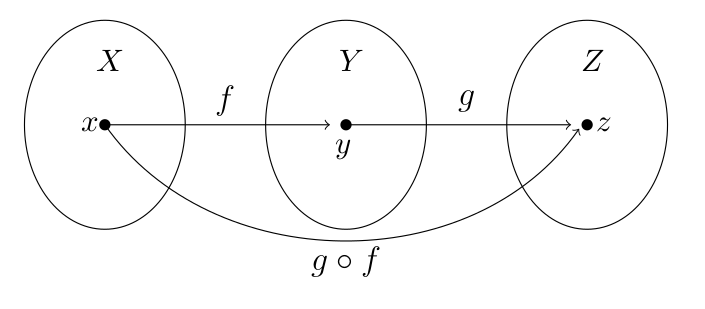
\includegraphics{./comp.png}

\begin{example}{} \label{Bsp:Komposition}
\item $f: \mathbb{R} \rightarrow \mathbb{R}$, $x\mapsto x^2$;~ $g:\mathbb{R} \rightarrow \mathbb{R}$, $x\mapsto \sin(x)$
\begin{align*}
g\circ f: \mathbb{R} &\rightarrow \mathbb{R} \\
x &\mapsto \sin(x^2) \\
f\circ g: \mathbb{R} &\rightarrow \mathbb{R} \\
x &\mapsto (\sin(x))^2
\end{align*}
\item Let $X$ be a set. Then $\operatorname{id}_X: X\rightarrow X$ with $x\mapsto x$ is called the \emph{identity map}.
If there is no confusion, one usually writes $\operatorname{id}$ instead of $\operatorname{id}_X$. 
Let $f: X\rightarrow X$ be a function. Then
\[
    f\circ \operatorname{id}=f=\operatorname{id}\circ f.
\]
\end{example}

